%Author Sujeendra R
\documentclass[12pt]{article}

\usepackage{fancybox}%for border and many more packages are not used

\usepackage{subfig}
\usepackage{wrapfig}
\usepackage{wasysym}
\usepackage{enumitem}
\usepackage{adjustbox}
\usepackage{ragged2e}    %packages imported which are required 
\usepackage[svgnames,table]{xcolor}
\usepackage{tikz}
\usepackage{longtable}
\usepackage{changepage}
\usepackage{setspace}
\usepackage{hhline}
\usepackage{multicol}
\usepackage{tabto}
\usepackage{float}
\usepackage{multirow}
\usepackage{makecell}
\usepackage{fancyhdr}
\usepackage[toc,page]{appendix}
\usepackage[hidelinks]{hyperref}
\usetikzlibrary{shapes.symbols,shapes.geometric,shadows,arrows.meta}
\tikzset{>={Latex[width=1.5mm,length=2mm]}}
\usepackage{flowchart}\usepackage[paperheight=11.69in,paperwidth=8.27in,left=0.98in,right=0.98in,top=0.98in,bottom=0.98in,headheight=1in]{geometry}
\usepackage[utf8]{inputenc}
\usepackage[T1]{fontenc}
\TabPositions{0.49in,0.98in,1.47in,1.96in,2.45in,2.94in,3.43in,3.92in,4.41in,4.9in,5.39in,5.88in,}

\urlstyle{same}

\setcounter{tocdepth}{5}
\setcounter{secnumdepth}{5}
 %setting boundry condition and margin parameters which are preset in ms word
\setlistdepth{9}
\renewlist{enumerate}{enumerate}{9}
		\setlist[enumerate,1]{label=\arabic*)}
		\setlist[enumerate,2]{label=\alph*)}
		\setlist[enumerate,3]{label=(\roman*)}
		\setlist[enumerate,4]{label=(\arabic*)}
		\setlist[enumerate,5]{label=(\Alph*)}
		\setlist[enumerate,6]{label=(\Roman*)}
		\setlist[enumerate,7]{label=\arabic*}
		\setlist[enumerate,8]{label=\alph*}
		\setlist[enumerate,9]{label=\roman*}

\renewlist{itemize}{itemize}{9}
		\setlist[itemize]{label=$\cdot$}
		\setlist[itemize,1]{label=\textbullet}
		\setlist[itemize,2]{label=$\circ$}
		\setlist[itemize,3]{label=$\ast$}
		\setlist[itemize,4]{label=$\dagger$}
		\setlist[itemize,5]{label=$\triangleright$}
		\setlist[itemize,6]{label=$\bigstar$}
		\setlist[itemize,7]{label=$\blacklozenge$}
		\setlist[itemize,8]{label=$\prime$}

\setlength{\topsep}{0pt}\setlength{\parindent}{0pt}
\renewcommand{\arraystretch}{1.3}





%start of the document
\begin{document}
%naming
\begin{Center}
{\fontsize{16pt}{19.2pt}\selectfont  \textbf{ SUJEENDRA\ R\ \   }{\fontsize{13pt}{15.6pt}\selectfont \textbf{\ \ \ \ \ \ \ \ \ \ \  }\par}\par}\par

\end{Center}


%image path must be specified
\begin{figure}[H]
	\begin{FlushRight}		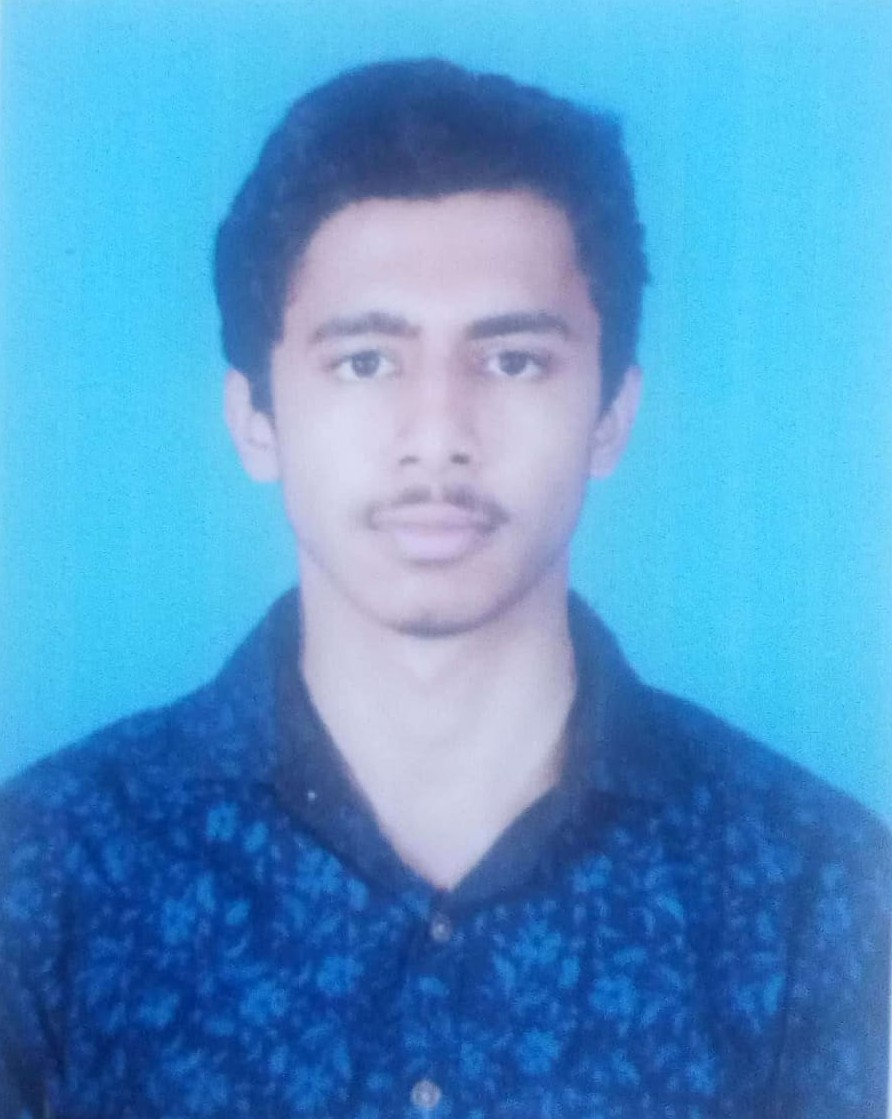
\includegraphics[width=1.08in,height=1.44in]{/home/sujeendra/Documents/Sujeendra_R_resume/Profile.jpeg}
	\end{FlushRight}\end{figure}



%address
\vspace{-4.2cm}

{\fontsize{13pt}{15.6pt}\selectfont \textbf{$\#$ 31 4\textsuperscript{th} A main CITB model}\par}\par

{\fontsize{13pt}{15.6pt}\selectfont \textbf{House Near Library Subhash Nagar}\par}\par

{\fontsize{13pt}{15.6pt}\selectfont \textbf{Karnataka Mysore-570007}\par}\par

{\fontsize{13pt}{15.6pt}\selectfont \textbf{Contact:7026335428}\par}\par

{\fontsize{13pt}{15.6pt}\selectfont \textbf{email id: sujeendrar.280@gmail.com}\par}


\vspace{\baselineskip}

\vspace{\baselineskip}

%objective
\vspace{\baselineskip}
{\fontsize{14pt}{16.8pt}\selectfont \textbf{Objective}\par}\par

{\fontsize{13pt}{15.6pt}\selectfont I have a keen interset in learning new topics ,so i would like to work on more Technical Projects like Eyantra ,especially on a subject like Robotics and Computer Vision.\par}\par


%for spacing between lines
\vspace{\baselineskip}
{\fontsize{14pt}{16.8pt}\selectfont \textbf{Education}\par}\par





%Education
\begin{table}[H]
 			\centering
\begin{tabular}{p{1.37in}p{1.37in}p{1.37in}p{1.38in}}
\hline
%1
\multicolumn{1}{|p{1.37in}}{\begin{Center}Degree\end{Center}} & 
\multicolumn{1}{|p{1.37in}}{\begin{Center}College/School\end{Center}} & 
\multicolumn{1}{|p{1.37in}}{\begin{Center}Passing Year\end{Center}} & 
\multicolumn{1}{|p{1.38in}|}{\begin{Center}Percentage\end{Center}} \\
\hhline{----}
%2
\multicolumn{1}{|p{1.37in}}{\begin{Center}SSLC\end{Center}} & 
\multicolumn{1}{|p{1.37in}}{\begin{Center}Marimallappa’s High School Mysore\end{Center}} & 
\multicolumn{1}{|p{1.37in}}{\begin{Center}2014\end{Center}} & 
\multicolumn{1}{|p{1.38in}|}{\begin{Center}97.44\end{Center}} \\
\hhline{----}
%3
\multicolumn{1}{|p{1.37in}}{\begin{Center}PUC\end{Center}} & 
\multicolumn{1}{|p{1.37in}}{\begin{Center}Marimallappa’s PU College Mysore\end{Center}} & 
\multicolumn{1}{|p{1.37in}}{\begin{Center}2016\end{Center}} & 
\multicolumn{1}{|p{1.38in}|}{\begin{Center}94\end{Center}} \\
\hhline{----}
%4
\multicolumn{1}{|p{1.37in}}{\begin{Center}B.E in Electronics and Communication\end{Center}} & 
\multicolumn{1}{|p{1.37in}}{\begin{Center}Sri Jayachamarajendra College of Enginnering(JSSTU)\end{Center}} & 
\multicolumn{1}{|p{1.37in}}{\begin{Center}2020\end{Center}} & 
\multicolumn{1}{|p{1.38in}|}{\begin{Center}CGPA on a scale of 10 .Five semester Score is\end{Center} \begin{Center}\par 9.3 \end{Center}\par } \\
\hhline{----}

\end{tabular}
 \end{table}
\end{document}